\section{Stoffwechsel}
\label{sec:stoffwechsel}
\subsection{Phototrophie}
\begin{description}
	\item[ATP-Produktion]	\hfill \\
	\item[Reduktion von Kohlenstoffdioxid]	\hfill	\\
		mit \ce{NADH} und \ce{NADPH},
		welche durch die vorherige Reduktion von \ce{NAD+} bzw. \ce{NADP*} erzeugt wurden.
\end{description}
Bei beiden Photosynthesevarianten finden
verschiedener akzessorischer Proteine und Photosystheme verwendung.
Dies ermöglich die Anpassung an verschiedene Lebensräume,
und die Anpassung an die vorhanden Lichtspektren.

\subsubsection{Oxygenen Photosynthese}
\begin{itemize}
	\item Kein zyklischer Elektronen Transport
	\item Z-Schema mit zwei Photosysteme, (II:P680;I:P700)
\end{itemize}

\subsubsection{Anoxygene Photosynthese}
\begin{itemize}
	\item zyklischer Elektronen Transport
	\item Ein Photosystem (P870)
	\item umgekehrter, energieverbrauchender Elektronentransport,
		wenn \ce{NAD(P)H} nötig
\end{itemize}

\subsubsection{\ce{CO2}-Fixierung}
\begin{description}
	\item[Calvin-Zyklus] ist am weitesten verbreitet.
		Mit den Schlüsselenzymen RUBISCO und Phosphoribulose-Kinase
		erfolgt die Bindung von \ce{CO2} in Glucose
		unter Verbrauch von \ce{ATP} und \ce{NADPH}.
		Siehe Abbildung \ref{fig:calvin_detail}.

	\item[Hydroxypropionat-Weg] der Grünen-Schwefelbakterien.
		Letzlich wird in zwei Zyklen zunächst zwei Moleküle \ce{CO2}
		in Form von Bicarbonat (\ce{HCO3-}) fetgelegt.
		Das Bicarbonat wird dann unter ATP und NADPH Verbrauch zu Glyoxalat aufgebaut.

		Anschließend werden zwei Glyoxalat Moleküle zu Pyruvat umgebaut.

	\item[umgekehrter Citrat-Zyklus] ist die Umkehrung des oxidativen Citratzyklus,
		deshalb auch reduktiver Citrat-Zyklus.
		Die Reaktionen innerhalb des oxidativen Zyklus werden dabei umgekehrt
		unter Umgehung bzw. der Verwenugn spezialisierter Moleküle für die 
		drei Unumkerhbahren Schritte des oxidativen Citrat-Zyklus.

\end{description}

\subsection{Glykolyse (EMP)}
\label{sec:glykolyse}
\begin{itemize}
	\item Ausgeglichene Oxidations-Reduktions-Reaktion
	\item Endprodukt Pyruvat
	\item Ausgangspunk für Fermentation und aerobe Atmung
	\item Weiter Produkte: Reduktionsäquivalent \ce{NADH+}
	\item Verbraucht: 2 ATP

\end{itemize}

\begin{enumerate}
	\item Stufe: Vorbereitende Reaktion
	\item Stufe: Synthese von ATP und Pyruvat
	\item Sutfe: Bildung von Fermentationsprodukten, aerobe Atmung
\end{enumerate}

\begin{figure}[htb!]
	\leavevmode
	\begin{center}
		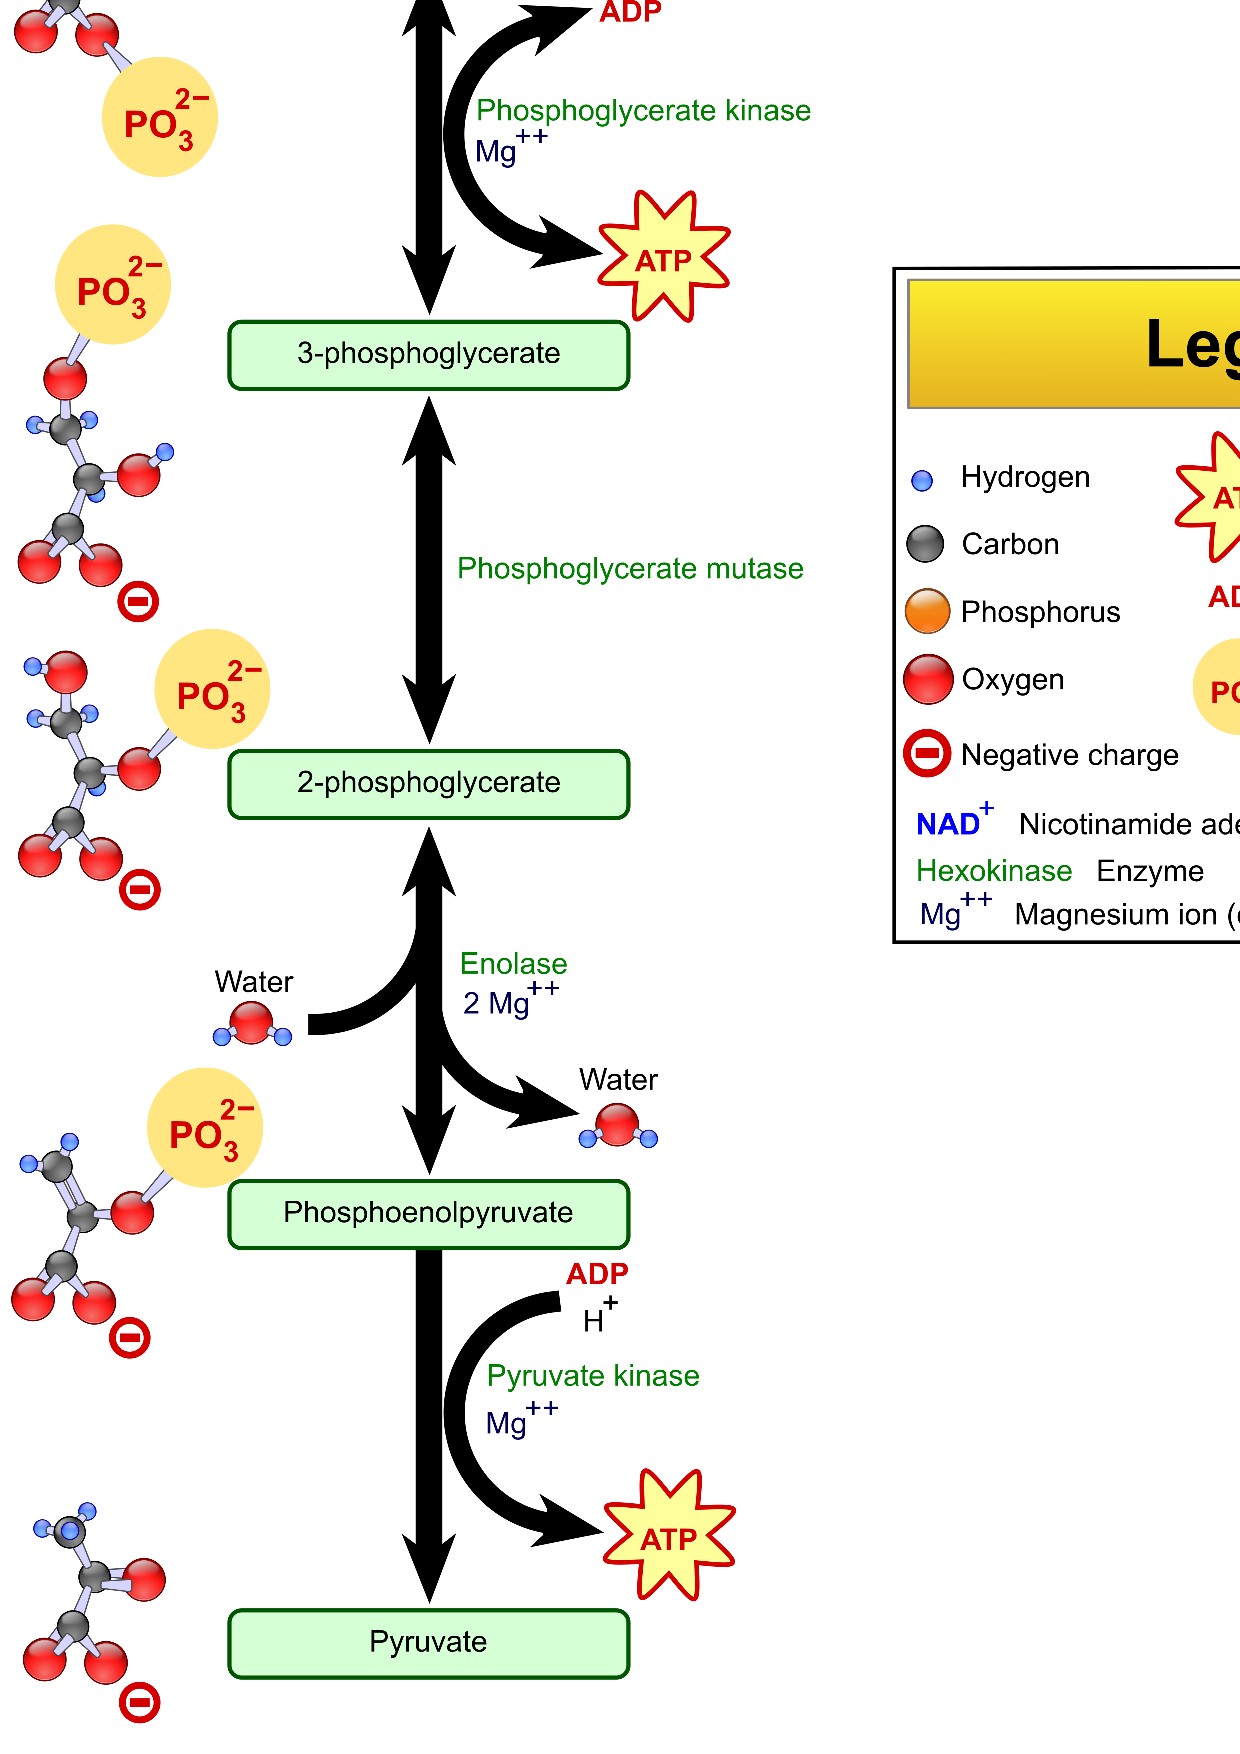
\includegraphics[scale=0.30]{./pictures/glykolysis_2k.pdf}
	\end{center}
	\caption{\slshape{Übersich über die Glykolyse.}}
	\label{fig:glykolyse}
\end{figure}

\subsection{Aerober Stoffwechsel}

\subsubsection*{Aerobe Atmung}
Die Anaerobe Atmung ist ein Stoffwechselvorgang,
zur Energieerzeung.
Durch oxidative biochemische Reaktionen wird dabei ATP erzeugt.
Sie fasst die folgenden Schritte zusammen:

\begin{description}
	\item[Gylkolyse]	\hfill	\\
		Siehe Abschnitt \ref{sec:stoffwechsel}.\ref{secglykolyse} 
		und Abbildung \ref{fig:glykolyse} auf Seite \pageref{fig:glykolyse}
	\item[oxdiative Decarboxylierung]	\hfill	\\
	\item[Citratzyklus]	\hfill	\\
		Siehe Abschnitt \ref{sec:citratzyklus}.
	\item[Endoxidation in der Atmungskette]	\hfill	\\
\end{description}

Die Gesamtbilanz lautet:
\begin{equation}
	\ce{C6H12O6} + 6\ \ce{O2} \rightarrow 6\ \ce{CO2} + 6\ \ce{H2O}
	\label{eq:aerobeAtmung}
\end{equation}

\subsection{Citratzyklus}
\label{sec:citratzyklus}

Der Citratzyklus ist ein zentraler Bestandteil bei der Veratmung organische Verbindungen.

\subsubsection*{Ablauf}
Der C\textsubscript{3}-Körper von Pyruvat wird decarboxyliert,
was zu einem Moleküle \ce{NADH} 
und einem mit dem Coenzym A gekoppelte Acetylmolekül führt.

Die Acetylgruppe von \textsl{Acetyl-CoA} geht mit der Vier-Kohlenstoff-Verbindung
\textsl{Oxalacetat} eine Verbindung ein,
was zur Bildung von \textsl{Citronensäure} führt,
woebi die Energie aus der Thioesterbindung im \textsl{Acetyl-CoA}
diese Synthese antreibt.
Es schließen sich Hydrierungs-, Decarboxylierungs- und Oxidationsreaktionen an
und zwei zusätzliche \ce{CO2}-Moleküle werden freigesetzt.
Zuletzt wird wieder \ce{Oxalacetat} gebildet
und kann seine Funktion als Acetylackezptor wieder übernehmen,
wodichr der Kreislauf vollendet wird.
\cite[S. 140]{brock}

\begin{figure}[ht!]
	\leavevmode
	\begin{center}
		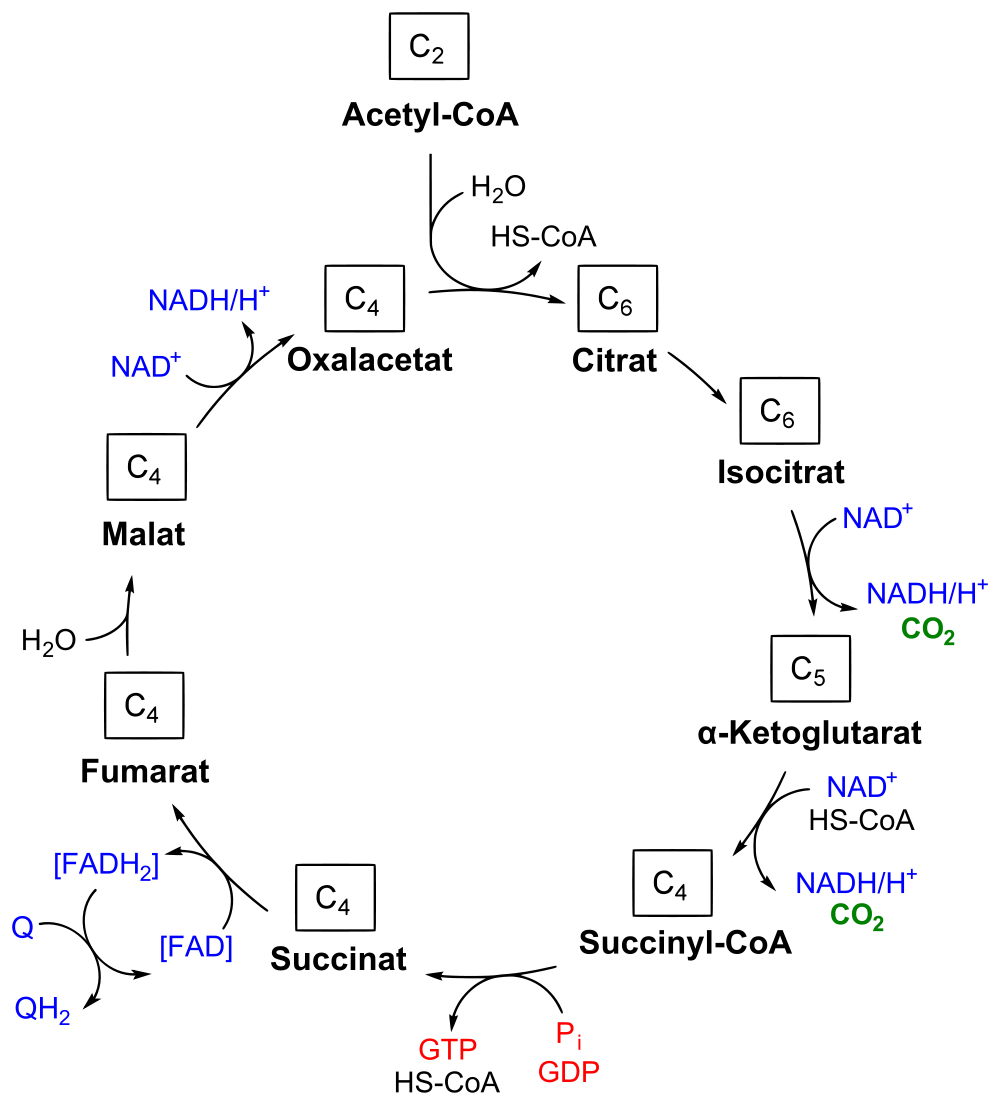
\includegraphics[scale=0.30]{./pictures/citratzyklus_1k}
	\end{center}
	\caption{Der Citrat-Zyklus.}
	\label{fig:calvinDetail}
\end{figure}

Die Zwischenprodukte des Citratzyklus sind auch wichtige Ausgangsstoffe für:
\begin{itemize}
	\item $\alpha$-Ketogularat, Oxalacetat \textrightarrow  div. Aminosäuren
	\item Succinyl-CoA \textrightarrow Porphyriniring der Cytochrome, Chlorophyll
	\item Oxalacetat \textrightarrow Phosphoenolpyriuvat (PEP)
	\item Acetyl-CoA \textrightarrow Fettsäurebiosythese
\end{itemize}

Die Gesamtausbeite beträgt bei Gylkolyse und Citratzyklus 38 ATP.
Wird ein Glukosemolekül fermentiert (Milchsäure-, oder Alkoholische-Gärung),
liegt der Energiegewinn bei nur 2 ATP.

Der Citratzyklus wird auch als Tricarbonsäure-Zyklus oder kurz TCA-Zyklus bezeichnet.

\subsection{Chemolithotrophie}
Neben den hier beschrieben Lebensweisen gibt es auch:

\begin{description}
	\item[Oxidation reduzierter Schwefelverbindungen] \hfill \\
		Reduzierte Schwefelverbindungen 
		und Schwefel sind sehr gute Protonendonnatoren für Chemolitotrophe.
		Schwefel- und Wasserstoff-Bakterien oxidieren diese Verbindungen
		und erzeugen damit eine protonenmotorische Kraft.
		Diese nutzen sie mit ATPasen zur Energiegewinnung.
		Sie fixieren dabei auch \ce{CO2} über den Calvinzyklus,
		was sie zu Autotrophen macht.

	\item[Eisenoxidation]	\hfill	\\
		Eisenbakterien können zweiwertiges Eisen als alleinige Energiequelle nutzen.
		Sie wachsen meist im Sauren 
		und sind oft mit Ausflüssen aus Erz- und Kohle-Gruben assoziert.
		Einiege phototrophe Purpurbakterien können
		anaerob oxidativ zweiwertiges in dreiwertiges Eisen umwandeln.

\end{description}

\subsubsection{Nitrifizeriung}
\begin{description}
	\item[Nitrosifizierer] oxidieren Ammoniak (\ce{NH3}) zu Nitrit (\ce{NO2-})
	\item[Nitrifizierer] oxidieren Nitrit (\ce{NO2-}) zu Nitrat (\ce{NO3-})
\end{description}

Bei der Ammoniakoxidation wird letztlich eine protonenmotorische Kraft
zur Energieerzeugung aufgebaut.
Dies geschieht über eine Elektronentransportkette.
Schlüsselenzyme sind hierbei die \emph{Ammoniakmonooxygenase},
welche Ammoniak zu Hydroxylamin und Wasser oxidiert,
und die \emph{Hydroxylaminoxidoreductase} die dann Hydroxylamin
zu Nitrit oxidert.
Dabei werden vier Elektronen abstrahiert.

Weiterhin gibt es noch dieAnaerobe Ammoniakoxidation (Anammox),
welche von den Mikroorganismen in einem mit membran bageschlossenen Kompartiment 
durchgeführt wird,
dem Anammoxosom.
Entdeckt wurde dieser Vorgang erst Anfang der 1980er Jahre an \emph{Brocadia anammoxidans}.
\\

\subsubsection{Wasserstoffoxidation}
Auch bei der Wasserstoffoxidation wird von den Chemolithotrophen Organismen
einen protonenmotorische Kraft aufgebaut.
Durch eine Hydrogenase wird das Wasserstoffgas gespalten
und die Elektronen in die Elektronentransportkette eingebracht.

\subsection{Anaerobe Lebensweise}
Neben den hier beschrieben Lebensweisen gibt es auch:
\begin{description}
	\item[Acetogenese]
	\item[Methanogenese]
\end{description}

\subsubsection{Anaerobe Atmung}
\subsubsection{Nitratreduktion}
\subsubsection{Sulfatreduktion}

\subsection{Fermentation}
\begin{itemize}
	\item inter ausbalacierte Oxidations-Reduktions-Reaktion
	\item keine externen e\textsuperscript{-}-Akzeptoren
	\item keine direkt mit Substratoxidation gekoppelte Elektronentransport-Phosphorylierung (kein prot.mot.Kraft)
	\item organische Verbindung als Substrate
	\item Ergebnis: reduizerte organische Verbindung
\end{itemize}

Zentrales Intermediat uach hier \textsl{Pyruvat}.

Glukoseabbau bei Fermetierern:
\begin{description}
	\item[``die meisten''] Embden-Meyerhof
	\item[Zymomonas]Entner-Doudroroff 
	\item[heterofermentative Milchsäureärung] Phosphoketolase
\end{description}


\subsubsection{Milchsäuregärung}

\begin{description}
	\item[Homofermentativ]	\hfill	\\
		\begin{itemize}
			\item Embden-Meyerhof-Parnas-Weg (Fruktose-1,6-Bisphoshat-Weg)
			\item Schlüsselenzym und Abschlussenzym: Laktat-Dehydrogenase
			\item Bilanz: Glukose \textrightarrow 2 Lactat + 2 ATP
		\end{itemize}

	\item[Heterofermentativ]	\hfill	\\
		\begin{itemize}
			\item Pentose-P-Weg
			\item Bilanz:
				\begin{description}
					\item[Leconostoc] Lactat + \ce{CO2} + \ce{EtOH}
					\item[Lactobacillus brevis] Lactat + \ce{CO2} + Acetat + Mannit
				\end{description}
		\end{itemize}
\end{description}

\subsubsection{Gemischte Säuregärung}

